\documentclass[tikz,border=6pt]{standalone}
\usepackage[T1]{fontenc}
\usepackage[utf8]{inputenc}
\usepackage{pgfplots}
\usepgfplotslibrary{groupplots}
\usetikzlibrary{calc}
\pgfplotsset{compat=1.18}
\begin{document}
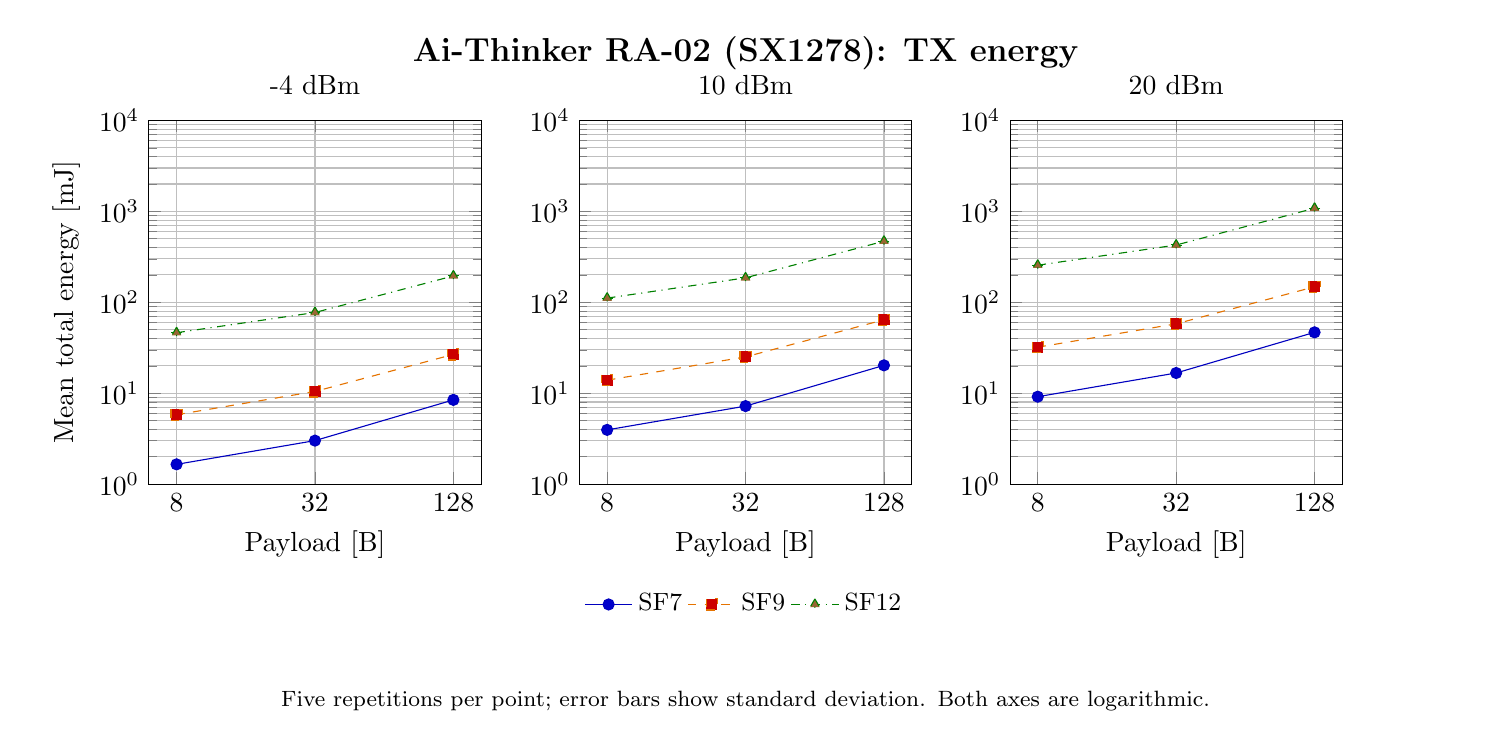
\begin{tikzpicture}
\begin{groupplot}[/pgf/number format/use comma, group style={group size=3 by 1, horizontal sep=1.25cm},
  width=5.8cm,height=6.2cm,xmode=log,log basis x=2,ymode=log,log basis y=10,ymin=1,ymax=10000,
  xtick={8,32,128},xticklabels={8,32,128},grid=both,xlabel={Payload [B]},
  legend style={draw=none,fill=none,font=\small,at={(0.5,-0.27)},anchor=north,legend columns=-1}]
% TX energy
\nextgroupplot[title={-4 dBm},ylabel={Mean total energy [mJ]}]
\addplot+[blue!75!black,solid,mark=*,error bars/.cd,y dir=both,y explicit] coordinates {(8,1.648305) +- (0,0.00325874833) (32,3.00636232) +- (0,0.00555323277) (128,8.43321329) +- (0,0.0084018148)};
\addplot+[orange!90!black,dashed,mark=square*,error bars/.cd,y dir=both,y explicit] coordinates {(8,5.79013274) +- (0,0.0122622964) (32,10.4363327) +- (0,0.0191395137) (128,26.6775518) +- (0,0.0536095294)};
\addplot+[green!50!black,dashdotted,mark=triangle*,error bars/.cd,y dir=both,y explicit] coordinates {(8,46.2285564) +- (0,0.0438460825) (32,77.1371382) +- (0,0.0244492514) (128,194.844658) +- (0,0.115106671)};
\nextgroupplot[title={10 dBm}]
\addplot+[blue!75!black,solid,mark=*,error bars/.cd,y dir=both,y explicit] coordinates {(8,3.94559521) +- (0,0.00261885689) (32,7.20505295) +- (0,0.00375114798) (128,20.228774) +- (0,0.00767127973)};
\addlegendentry{SF7}
\addplot+[orange!90!black,dashed,mark=square*,error bars/.cd,y dir=both,y explicit] coordinates {(8,13.8888749) +- (0,0.0120913868) (32,25.0627454) +- (0,0.024065589) (128,64.1550056) +- (0,0.0507594555)};
\addlegendentry{SF9}
\addplot+[green!50!black,dashdotted,mark=triangle*,error bars/.cd,y dir=both,y explicit] coordinates {(8,111.055711) +- (0,0.0341872035) (32,185.64329) +- (0,0.0760682488) (128,469.169338) +- (0,0.125790936)};
\addlegendentry{SF12}
\nextgroupplot[title={20 dBm}]
\addplot+[blue!75!black,solid,mark=*,error bars/.cd,y dir=both,y explicit] coordinates {(8,9.14263173) +- (0,0.033071013) (32,16.6662982) +- (0,0.0759317298) (128,46.6681595) +- (0,0.265770359)};
\addplot+[orange!90!black,dashed,mark=square*,error bars/.cd,y dir=both,y explicit] coordinates {(8,32.0362344) +- (0,0.191695646) (32,57.8914051) +- (0,0.301160929) (128,147.93604) +- (0,0.575817552)};
\addplot+[green!50!black,dashdotted,mark=triangle*,error bars/.cd,y dir=both,y explicit] coordinates {(8,255.430656) +- (0,0.504895344) (32,425.990612) +- (0,1.52714045) (128,1081.92533) +- (0,2.43314516)};
\end{groupplot}
\node[font=\bfseries\large] at ($(group c2r1.north)+(0,0.85cm)$) {Ai-Thinker RA-02 (SX1278): TX energy};
\node[font=\footnotesize,align=center,text width=18cm] at ($(group c2r1.south)+(0,-2.75cm)$) {Five repetitions per point; error bars show standard deviation. Both axes are logarithmic.};
\end{tikzpicture}
\end{document}
